\documentclass[
            a4paper
            ]{scrartcl}%article

\usepackage{style}

\title{Dependable Systems}
\author{}
\subtitle{Ausarbeitung der gesammelten Prüfungsfragen}
\rohead{Dependable Systems}
\subject{VU Dependable Systems 182.712}

\begin{document}

\maketitle

{
  \hypersetup{linkcolor=black}
  \tableofcontents
}

\newpage
%to start with section 2
\setcounter{section}{1}

\section{Kapitel: Basic concepts and terminology}
\subsection[Was bedeutet Dependability?]{Was bedeutet Dependability?\\{\itshape\smaller[2] 7.2013, Ausarb. 2009}}
Dependability\footnote{Dependability: Systemstabilität, Zuverlässigkeit} ist die Verlässlichkeit eines Computersystems, so dass es
vertretbar ist sich auf die zur Verfügung gestellten Services zu verlassen.

\textbf{Reliance}\footnote{Reliance: Verlass, Vertrauen}: Man kann sich darauf verlassen, dass
\begin{itemize}
    \item sich das System gemäß den Spezifikationen verhält
    \item das   System  Hazards\footnote{Hazard: Gefahr, Riskio} (=Verhalten,   das   zu   unerwünschten   
        Konsequenzen führt) verhindert
\end{itemize}

Je näher die Servicespezifikation und das Risiko(Hazard) sind, desto höher ist der
Gefährlichkeitsgrad des Systems.
$\Rightarrow$ Anwendungsspezifischer Fehlertoleranzrahmen.

\subsection[Dependability Attribute (Parameter)]{Dependability Attribute (Parameter)\\{\itshape\smaller[2] 7.2013, Ausarb. 2009}}
\minisec{Reliability (Funktionsfähigkeit)}
Verlässlichkeit bezogen auf Kontinuität des Service.  $R(t)$  ist die
Wahrscheinlichkeit, dass 
das System über eine Periode $t$ hinweg ununterbrochen zur Verfügung steht.

\[R(0)=1, R(\infty)=0\]

Bei einer konstanten Fehlerrate sieht sie wie folgt aus:
\[R(t)=e^{-\lambda t}\]
\minisec{Availability (Verfügbarkeit)}
Verlässlichkeit bezogen auf die Verfügbarkeit zu einem bestimmten Zeitpunkt: $A$
oder $V$ ist 
der Prozentsatz der Zeit, zu dem das System gemäß den Spezifikationen
funktioniert.

\minisec{Safety (Sicherheit)}
Verlässlichkeit   bezogen   auf   das   Vermeiden   katastrophaler
Auswirkungen: $S(t)$ ist die 
Wahrscheinlichkeit, dass ein bestimmtes katastrophales Verhalten innerhalb einer
Periode $t$ 
nicht auftritt.

Die nicht Erreichbarkeit von Zuständen, die zu Tod, Verletzung, Schaden, Berufskrankheit, oder zu einem Verlust von Gerät oder Besitz führen.
Safety ist ein relativer Begriff.

\minisec{Security (Vertraulichkeit)}
Verlässlichkeit bezogen auf das Verhindern von unerlaubtem Zugriff auf
Informationen.
\begin{itemize}
    \item Secrecy\footnote{secrecy: Geheimhaltung}: wer kann Daten lesen
    \item Integrity\footnote{integrity: Integrität, Unbescholtenheit}: wer kann
        Daten ändern und wie?
    \item Availability\footnote{availability: Verfügbarkeit}: für wen ist es möglich, die Verfügbarkeit eines Systems zu verringern
\end{itemize}
\minisec{Weitere:}
    Usability (Verwendbarkeit), Recoverability (Wiederherstellbarkeit),
Maintainability (Wartbarkeit), Extendability (Erweiterbarkeit), \ldots

\subsection[Reliability vs Safety]{Reliability vs Safety\\{\itshape\smaller[2] 7.2013, Ausarb. 2009}}
Reliability wird durch die Verlässlichkeit des kontinuierlichen Services und der funktionalen Spezifikation des Services beschrieben, 
Safety wird durch eine nicht funktionale Spezifikation beschrieben. Sie ist die Verlässlichkeit der Verhinderung von Katastrophalen Konsequenzen. Das bedeutet, die Verhinderung von \textbf{Hazards}.\\

Safety $\subseteq$ Reliability\\

Die Auswirkungen einer Safety-Verletzung sind im Gegensatz zu den Auswirkungen
einer 
Reliability-Verletzung katastrophal.
Das bedeutet die Fehler kosten unterschiedlich viel Geld.

Um Safety bzw. Reliability zu erreichen werden unterschiedliche
Methoden des 
Systemdesigns angewandt. Oft stehen die Ziele in \textbf{Konflikt} miteinander (z.B.
Zugsignale: alle 
Ampeln   auf   rot   ist   sicher,   aber   kein   Zug   kann   fahren,
wodurch   das   Zugsystem   nicht 
funktionsfähig ist).

Wenn es keinen sicheren, nicht-funktionalen Systemzustand gibt (d.h. das System
ist  \textbf{fail-operational}), sind Safety und Reliability jedoch eng verwandt (z.B.
Fly-by-Wire). Denn nach dem Start gibt es keinen safe (nicht-funktionierenden)
system state.

\subsection[Reliability vs Availability]{Reliability vs Availability\\{\itshape\smaller[2] 7.2013, Ausarb. 2009}}
Availability ist als Kenngröße nur dann relevant, wenn die Möglichkeit der
Wartung existiert. 

\minisec{Beispiele}
Bei einem Mars-Rover muss die Missions-Reliability möglichst hoch sein, da das
System ab 
dem ersten Ausfall für immer unbrauchbar wird. 

Ein System zur automatisierten Montage muss 
jedoch eine gewisse Anzahl an Stücken pro Jahr produzieren, die Availability ist
daher der wichtigste Parameter, denn dieses System kann notfalls zur Wartung
auch abgeschalten werden.

\subsection[Wie hoch ist die Availability in einem System, das nicht gewartet wird?]{Wie hoch ist die Availability in einem System, das nicht gewartet wird?\\{\itshape\smaller[2] 7.2013, Ausarb.
2009}}
Ist ein System ab dem ersten Ausfall nie wieder einsatzfähig, beträgt die
Availability Null:
\[A = \frac{\text{Zeitdauer der Einsatzfähigkeit}}{\text{Zeitdauer der
Einsatzfähigkeit} + \text{Zeitdauer der nicht Einsatzfähigkeit}} =
\frac{<\infty}{(<\infty)+\infty} = \frac{<\infty}{\infty} = 0\]
\[\frac{\text{MTTF}}{\text{MTTF}+\text{MTTR}}\]

\subsection[Spezifikation]{Spezifikation\\{\itshape\smaller[2] Ausarb. 2009}}
Alle Attribute der Dependability basieren auf einer Spezifikation. Die
Spezifikation und die Analyse   des   möglichen   Verhaltens   eines   Systems   und   dessen
Auswirkungen   sind   die 
schwierigsten Aufgaben beim Design eines dependable Systems.

Eine gute Spezifikation ist:
\begin{itemize}
\item exakt
\item konsistent
\item vollständig
\item verbindlich (authoritative)
\end{itemize}
Oft   werden   Spezifikationen   auf   unterschiedlichen   Ebenen   verwendet,
z.B.   funktionelle,  Reliability-, Safety-Ebene

\newpage
\section{Kapitel: Fault-tolerance and Modeling}
\subsection[Failure Probability \& Reliability]{Failure Probability \& Reliability\\{\itshape\smaller[2] Ausarb. 2017}}
Die \textbf{Failure Probability} $Q(t)$ (Fehlerwahrscheinlichkeit) ist die Wahrscheinlichkeit, dass ein System in einer Zeitspanne $[0:t]$ \textbf{nicht} nach der Spezifikation verhält.\\
Die \textbf{Reliability} $R(t)$ (Zuverlässigkeit eines Systems) ist die Wahrscheinlichkeit, dass ein System in einer Zeitspanne $[0:t]$ nach der Spezifikation verhält.
\[R(t)=1-Q(t)\]
\begin{figure}[H]
\centering
	\begin{tikzpicture}
		\pgfplotsset{
				scale only axis,
				domain=0:12.5,
				xmin=0, xmax=12.5,
        samples=50,
        height=5cm,
        width=14cm,
        clip=false,
				xtick={0,12.5},
				xticklabels={$0$,$\infty$},
		}

		\begin{axis}[
			axis y line*=left,
			ymin=0, ymax=1,
			xlabel=Time t,
			ylabel=Reliability $R(t)$,
			ytick={0,0.2,0.4,0.6,0.8,1},
			yticklabels={0,0.2,0.4,0.6,0.8,1},
			ylabel near ticks
		]
		\addplot[thin, smooth, black] {1-(5/(5+1494*exp(-0.95*x)))};
		\end{axis}

		\begin{axis}[
			axis y line*=right,
			hide x axis,
			ymin=0, ymax=1,
			ylabel=Failure Probability $Q(t)$,
			ylabel near ticks,
			ytick={0,0.2,0.4,0.6,0.8,1},
			yticklabels={1,0.8,0.6,0.4,0.2,0}
		]
		\end{axis}
	\end{tikzpicture}
	\caption{Reliability \& Failure Probability}%
	\label{fig:reliability_failurePropability}%
\end{figure}

\subsection[Warum werden beim Modellieren von zuverlässigen Systemen gerne
    konstante Fehlerraten angenommen?]{Warum werden beim Modellieren von zuverlässigen Systemen gerne
    konstante Fehlerraten angenommen? \\{\itshape\smaller[2] 2010}}
    Die \textbf{Fehler-Dichtefunktion} $f(t)$ zum Zeitpunkt $t$ ist die Anzahl der Fehler
    im Zeitabschnitt $\Delta t$:
    \[f(t)=\frac{dQ(t)}{dt}=-\frac{dR(t)}{dt}\]
    wobei hier $Q(t)$ die Fehlerwahrscheinlichkeit angibt.
    Die \textbf{Fehlerrate} $\lambda(t)$ ist definiert als die Anzahl der Fehler im Zeitabschnitt
    $\Delta t$, mit der Einheit FIT (failures in time), in Bezug auf die Anzahl der korrekten Komponenten zum Zeitpunkt
    $t$:
    \[\lambda(t)=\frac{f(t)}{R(t)}=-\frac{dR(t)}{dt}\frac{1}{R(t)}\]

    Im Fall von konstanten Fehlerraten ($\lambda(t)=\lambda$) ist es so dass die Reliability definiert
    werden kann, als $R(t)=e^{-\lambda t}$. Damit lautet die Failure Density (Fehlerdichte):
    \[f(t)=\frac{d R(t)}{dt}=-\lambda e^{-\lambda t}\]

    Das bedeutet, es ist viel einfacher zu berechnen. Außerdem können die Fehlerraten aus bekannten Bauteilen aus
    den dazugehörigen Spezifikationen ausgelsen werden und direkt in der Formel verwendet werden.
    Außerdem werden von einigen Modellen (z.B. Markov-Modellen) nur konstante Fehlerraten unterstützt.

    Wenn die Fehlerraten mit der Zeit zu oder abnehmen, kann auch die \textbf{Weibull
    verteilte Fehlerrate} verwendet werden:
    Dabei wird die Variable $\alpha$ eingeführt: 
    \begin{enumerate}
        \item $\alpha<1$ Fehlerrate fällt mit der Zeit
        \item $\alpha=1$ konstante Fehlerrate
        \item $\alpha>1$ Fehlerrate steigt mit der Zeit
    \end{enumerate}
    In diesem Fall ist $\lambda$ definiert, als ($\lambda(t)=\alpha\lambda(\lambda t)^{\alpha-1}$) und somit gilt für $R(t)=e^{-(\lambda t)^\alpha}$.
    \[f(t)=\frac{d R(t)}{dt}=-\alpha\lambda(\lambda t)^{\alpha-1} e^{-(\lambda t)^{\alpha}}\]
\begin{figure}[H]
    \centering
    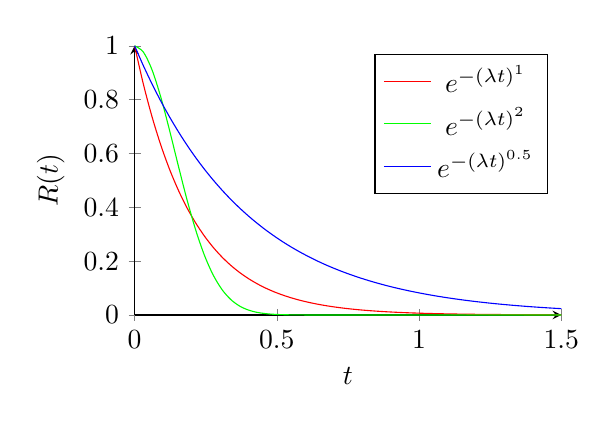
\begin{tikzpicture}
    \begin{axis}[
        domain=0:1.5,
        axis x line=bottom, % no box around the plot, only x and y axis
        axis y line=left, % the * would suppress the arrow tips
        ylabel={$R(t)$},
        xlabel={$t$},
        legend pos=north east,
        samples=50,
        height=5cm,
        width=7cm,
        clip=false]
        \addplot[thin, smooth, red] {exp(-5*x)};
        \addlegendentry[align=left]{$e^{-(\lambda t)^1}$};

        \addplot[thin, smooth, green] {exp(-(5*x)^2)};
        \addlegendentry[align=left]{$e^{-(\lambda t)^2}$};

        \addplot[thin, smooth, blue] {exp(-5*x)^0.5};
        \addlegendentry[align=left]{$e^{-(\lambda t)^{0.5}}$};
    \end{axis}
    \end{tikzpicture}
    \caption{Weibull verteilte Fehlerrate}
\end{figure}

In Halbleiteranwendungen wird häufig die \textbf{Logarythmischnormalverteilte Fehlerrate} verwendet. Diese passt sich gut an die Halbleiterlebensdauer an.
\subsection[Wahrscheinlichkeitstheoretische Modellierung]{Wahrscheinlichkeitstheoretische Modellierung\\{\itshape\smaller[2] 7.2013, Ausarb. 2009}}
Zur Vereinfachung werden die folgenden Annahmen gemacht: 
\begin{itemize}
	\item Die Teilkomponenten sind unterscheidbar
	\item Jede Komponente hat eine eigene Fehler-/Reperaturrate
	\item Modell basiert auf den Verbindungen der einzelnen Komponenten
\end{itemize}
\subsubsection{Was gehört dazu?}
    Simple Blockdiagram, Arbitrary\footnote{arbitrary: frei, beliebig, willkürlich} Blockdiagram, Markov Model, General Stochastic Petri Net
    \subsubsection{Simple Block Diagram}
    Modellierung beliebiger Kombinationen von seriell und parallel verbundenen Komponenten.
    \minisec{Für serielle Verbindungen gilt:} die Reliability nimmt ab, je mehr Komponenten seriell geschaltet werden:
    \[R_{seriell}(t)=\prod_{i=1}^n R_i(t)\]
    \[Q_{seriell}(t)=1-R_{seriell}=1-\prod_{i=1}^n R_i(t)=1-\prod_{i=1}^n (1-Q_i(t))\]
    \minisec{Für parallele Verbindungen gilt:} die Reliability nimmt zu, je mehr Komponenten parallel geschaltet werden:
    \[Q_{parallel}(t)=\prod_{i=1}^n Q_i(t)\]
    \[R_{parallel}(t)=1-Q_{parallel}=1-\prod_{i=1}^n Q_i(t)=1-\prod_{i=1}^n (1-R_i(t))\]
    \minisec{Vorteil:} 
    \begin{itemize}
        \item leichte Berechnung für konstante Failure-Raten
    \end{itemize}
    \minisec{Nachteile:} 
    \begin{itemize}
        \item implizite Annahme der Unabhängigkeit von Fehlern
        \item Wartung kann nicht modelliert werden
        \item es können nur parallele oder serielle Verbindungen modelliert werden
        \item es kann nur aktive Redundanz unter der Annahme von Fail-Silence modelliert werden
    \end{itemize}
		
    \begin{figure}[H]
    \centering
    \includegraphics[page=15, width=0.2\linewidth,angle=-90,clip=true,trim=200 120 200 270]{DCS-2012-P3}
    \caption{Simple Blockdiagramm}
    \end{figure}

    \subsubsection{Arbitrary Block Diagram}
    Wie Simple Block Diagram, aber die Beschränkung auf serielle und parallele Verbindungen fällt weg. Unter anderem sind damit Voting Systeme und passive Redundanz möglich.\\
		
\begin{figure}[H]
    \centering
    \includegraphics[page=16, width=0.2\linewidth,angle=-90,clip=true,trim=200 50 200 400]{DCS-2012-P3}
    \caption{Arbitrary Block Diagramm}
\end{figure}

    Hierbei wird bei der Berechnung der Reliability das Inklusions-Exklusionsprinzip angewandt:
    \[R_{block}(t)=R_{AB}+R_{BE}+R_{DE}+R_{CD}-R_{ABE}-R_{ABCD}-R_{BDE}-R_{CDE}+R_{ABCDE}\]
    Wobei beispielsweise $R_{ABC}$ definiert ist als:
    \[R_{ABC} = R_{seriell}(A,B,C)\]

    \subsubsection{Markov Modell}
    \minisec{Geeignet zum Modellieren von}
        \begin{itemize}
        \item Allgemeinen Strukturen (aktive und passive Redundanz, Voting-Redundanz)
        \item Systemen   mit   komplexen   Abhängigkeiten   (Fehler   müssen   nicht   als   unabhängig angenommen werden
        \item Coverage Effects
				\item Maintenance von Systemen
        \end{itemize}
    \minisec{Einschränkungen}
        \begin{itemize}
        \item Markov Property:  Das Verhalten des Systems  ist unabhängig  von seiner Geschichte 
(abgesehen vom vorhergehenden Zustand)
        \item nur konstante Failure-Rates
        \end{itemize}
    \minisec{Design}
        Identifikation von relevanten Zuständen, Übergänge zwischen den Zuständen erkennen und anschließende Konstruktion des Markovgraphen.
    \minisec{Evaluierung}
        Aufstellen der Differentialgleichungen, anschließends lösen (z.B. mit SHARPE) für Reliability $R(t)$

        Die Integration der Differentialgleichungen ergibt die MTTF.

    \begin{figure}[H]
    \centering
    \includegraphics[page=31, width=0.2\linewidth,angle=-90,clip=true,trim=330 380 80 80]{DCS-2012-P3}
    \caption{Markov-Modell von 2 parallelen Komponenten}
    \end{figure}

    \begin{figure}[H]
    \centering
    \includegraphics[page=32, width=0.1\linewidth,angle=-90,clip=true,trim=250 380 200 80]{DCS-2012-P3}
    \caption{Übergänge identischer Komponenten (gleiche Failure Rates) zusammenfassen}
    \label{fig:zusammenfassung}
    \end{figure}
    z.B: die Differentialgleichungen aus \Fref{fig:zusammenfassung}:
    \begin{eqnarray*}
        \frac{dP_1(t)}{dt}=&-2\lambda P_1(t) &+ \mu P_2(t)\\
        \frac{dP_2(t)}{dt}=&-2\lambda P_1(t) &- (\lambda+\mu)P_2(t)\\
        \frac{dP_3(t)}{dt}=& &+ \lambda P_2(t)
    \end{eqnarray*}
    Die MTTF wäre dann wie folgt:
    \[MTTF = \int_{t=0}^\infty\left(P_1(t)+P_2(t)\right)dt=T_1+T_2\]
    Mit den folgenden Grenzwahrscheinlichkeiten: 
        \begin{itemize}
            \item $P_1(0)=1$
            \item $P_2(0)=0$
            \item $P_3(0)=0$
            \item $P_1(\infty)=0$
            \item $P_2(\infty)=0$
            \item $P_3(\infty)=1$
        \end{itemize}

\subsubsection[Markoveigenschaft]{Markoveigenschaft\\{\itshape\smaller[2] Ausarb. 2009}}
Das   Verhalten   des   Systems   ist   zu   jedem   Zeitpunkt   unabhängig   von   der   Vorgeschichte, 
abgesehen vom letzten Zustand.

\subsubsection{General Stochastic Petri Net (GSPN)}
Erweiterung von basic Petri Nets: Übergangs-delays können deterministisch gleich Null oder 
Zufalls-variablen unterschiedlichster Verteilungen (z.B. exponentiell) sein.

GSPNs sind isomorph zu kontinuierlichen Markov-Ketten (d.h. alles was mit Markov-Ketten 
modelliert   werden   kann,   kann   auch   mit   GSPNs   modelliert   werden   und   umgekehrt), 
allerdings   bieten   sie   wesentlich   mehr   Mechanismen,   sodass   allgemeine   Systeme, 
Algorithmen und Prozesse leichter modelliert werden können. Im Gegensatz dazu werden 
Markov-Ketten für große Systeme schnell sehr komplex.

Die  Konvertierung  von GSPNs in  Markov-Ketten  sowie  deren  Auswertung  kann komplett 
automatisiert erfolgen.

Die folgenden Schritte müssen durchgeführt werden:
        \begin{itemize}
            \item Modellkonstruktion (bottom-up oder top-down)
            \item Modellvalidierung (strukturelle analyse, formale Beweise)
            \item Definition von Markings und Transition-Fireings.
            \item Konvertierung zur Markovkette (kann automatisiert erfolgen)
            \item Lösung der Markovkette
        \end{itemize}

%TODO: wie kann man überprüfen, ob das Modell der Spezifikation entspricht? 



\subsection[Modellierung für Software]{Modellierung für Software\\{\itshape\smaller[2] Ausarb. 2017}}
\textbf{Probabilistic Structural Modeling}  ist für Software nicht gut geeignet, da es bei Software 
keine ausreichend definierten individuellen Komponenten gibt, die Komplexität sehr hoch ist, 
keine  \textbf{Unabhängigkeit der Fehler}  angenommen werden kann (da nur eine CPU und ein 
Speicherbereich   für   verschiedene   Prozesse   existiert),   Aspekte   der   Echtzeitverarbeitung 
nicht modelliert werden können und Parallelität und Synchronisierung nicht beachtet werden (außer bei GSPNs).
Das \textbf{Reliability Growth Model} ist besser für die Modellierung von Software geeignet.

\subsection[Reliability Growth Model]{Reliability Growth Model\\{\itshape\smaller[2] Ausarb. 2017, Ausarb. 2009}}
Reliablility Growth Models basieren auf der Idee einer iterativen Verbesserung nach dem Schema testing $\rightarrow$  correction $\rightarrow$ re-testing

Dabei werden keine Annahmen über die System-Struktur (insbesondere über die Aufteilung 
in Komponenten) getroffen.

Z.B. Software Reliability Growth:
Software-Test  $\rightarrow$  Aufzeichnen der Zeitperioden zwischen aufeinander folgenden Fehlern  $\rightarrow$
ausbessern der Fehler

Ausgehend von den gemessenen Zeiträumen (Perioden) kann auf die zukünftigen Perioden 
zwischen zwei Fehlern geschlossen werden (und z.B. als MTTF angegeben werden)
\minisec{Ziele:}
\begin{itemize}
\item Disziplinierte und kontrollierte Verbesserung der Reliability
\item Extrapolieren von zukünftiger Reliability auf Basis der aktuellen Reliability
\item Abschätzen des Aufwands für Test, Verbesserung und Re-Test
\end{itemize}
\minisec{Vorteile:}
\begin{itemize}
\item Erlaubt Modellierung von alterungsbedingten Fehlern und Design-Fehlern
\item Kann für Hardware und für Software eingesetzt werden
\end{itemize}
\minisec{Nachteile:}
\begin{itemize}
\item Die Zuverlässigkeit dieses Modells variiert stark
\end{itemize}

Beim Testen der Software werden die Zeiten zwischen den Fehlern $t_1, t_2, ...,t_i$ gespeichert und von diesen Zeiten abhängig wird die Vorhersage von $T_i$=MTTF (und naturlich auch $T_{i+1}, T_{i+2}, ...$) gemacht.

\subsection[Assumption Coverage]{Assumption\footnote{assumption: Annahme, These, Vermutung} Coverage\\{\itshape\smaller[2] 7.2013, Ausarb. 2009}}
Unter der Abdeckung (Coverage) eines Fehlermodells versteht man die Anzahl von Fehlern, die im Modell beschreibbar sind, zu der Anzahl von tatsächlich auftretenden Fehlern. 

    Jedes Modell/Design basiert auf einer Menge von Annahmen über das Verhalten der Komponenten in der Umgebung. Die Assumption Coverage ist die Wahrscheinlichkeit, dass die Annahmen der realen Welt entsprechen. 

    Die berechnete Reliability eines Systems muss immer mit der Assumption
    Coverage 
    multipliziert   werden.   
    Dadurch   kann   die   Reliability   oft
    empfindlich   reduziert   werden.   Ein 
    System mit perfekter Reliability ist immer nur so gut wie die Assumption
    Coverage, die der 
    Berechnung der Reliability zugrunde liegt.
		

\minisec{Error Detection Coverage} (bei aktiver Redundanz)
Wie viel Prozent der Fehler einer 
Komponente werden von einem Switch erkannt, so dass dieser zur funktionierenden 
Komponente umschalten kann.

\minisec{Fault Hypotesis} (oder Fault Assumption)
Gibt an welche Fehler von einem Server gehandhabt werden müssen.

\minisec{Failure Semantics}
Server können Fehler nur behandeln, wenn die Wahrscheinlichkeit, dass der Fehler nicht behandelt wird niedrig genug ist.

Daraus ergibt sich, dass die Assumtion Coverage die Wahrscheinlichkeit angibt, dass ein Fehler Zustand, definiert in der Failure Semantic, die Wirklichkeit abdeckt.

    \textbf{Beispiel}:  \textbf{2-Aktive-Redundanz}  (zwei   parallel   geschaltete   
    Komponenten)
    vs.  \textbf{TMR}  (Triple 
    Modular  Redundancy):   Reliability   von   2-Aktiver-Redundanz  höher,
    beruht   jedoch   auf   der 
    Annahme, dass sich die Komponenten \textbf{fail-silent} verhalten. TMR beruht auf der
    Annahme, 
dass   sich   Komponenten  \textbf{fail-consistent}  verhalten,   was   einer
    Assumption-Coverage   von 
    annähernd 1 entspricht (byzantinische Fehler sind sehr selten).

    Das bedeutet, die Assumption-Coverage von einem Active-Redundant System muss immer kleiner als 1 sein.

\begin{figure}[H]
    \centering
    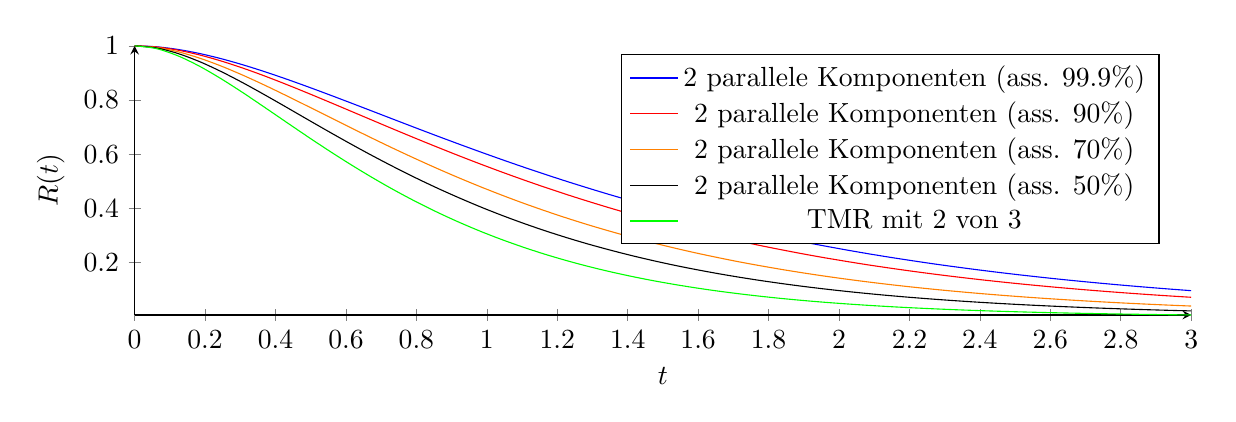
\begin{tikzpicture}
    \begin{axis}[
        domain=0:3,
        axis x line=bottom, % no box around the plot, only x and y axis
        axis y line=left, % the * would suppress the arrow tips
        ylabel={$R(t)$},
        xlabel={$t$},
        legend pos=north east,
        samples=50,
        height=5cm,
        width=15cm,
        clip=false]
        %\addplot[thin, smooth, red] {exp(-x)};
        %\addlegendentry[align=left]{1 Komponente};

        \addplot[thin, smooth, blue] {1-(1-exp(-1.001*x))^2};
        \addlegendentry[align=left]{2 parallele Komponenten (ass. 99.9\%)};

        \addplot[thin, smooth, red] {1-(1-exp(-1.1*x))^2};
        \addlegendentry[align=left]{2 parallele Komponenten (ass. 90\%)};

        \addplot[thin, smooth, orange] {1-(1-exp(-1.3*x))^2};
        \addlegendentry[align=left]{2 parallele Komponenten (ass. 70\%)};

        \addplot[thin, smooth, black] {1-(1-exp(-1.5*x))^2};
        \addlegendentry[align=left]{2 parallele Komponenten (ass. 50\%)};

        \addplot[thin, smooth, green] {exp(-x)^3+3*(exp(-x)^2)*(1-exp(-x))};
        \addlegendentry[align=left]{TMR mit 2 von 3};
    \end{axis}
    \end{tikzpicture}
    \caption{Assumption Coverage}
\end{figure}

\subsection[Was bedeutet Coverage beim Markov-Graphen?]{Was ist Coverage allgemein und was bedeutet sie beim Markov-Graphen?\\{\itshape\smaller[2] Ausarb. 2009}}

    \begin{figure}[H]%TODO: was ist das
    \centering
    \includegraphics[page=37, width=0.1\linewidth,angle=-90,clip=true,trim=350 200 100 200]{DCS-2012-P3}
    \caption{2-Active-Rundant System (Assumption Coverage $c$, Failure Rate $\lambda$)}
    \label{fig:actv_red}
    \end{figure}
		
Beim Markov- Graph muss die Coverage entsprechend berücksichtigt werden. D.h. die Wahrscheinlichkeit das der Fehler innerhalb der fault-semantic liegt muss bei den "`normalen"' Übergängen berücksichtigt werden. Mit der Gegenwahrscheinlichkeit führt dann zusätzlich noch eine Kante direkt zum Fehlzustand. 

\newpage
\section{Kapitel: Processes and Certification Standards}
\subsection[Probability/Severity]{Probability/Severity\\{\itshape\smaller[2] Ausarb. 2009}}
Das   primäre   Ziel   von   Safety   ist   eine   umgekehrt   proportionale   Beziehung   zwischen 
Wahrscheinlichkeit und Schwere eines Fehlers herzustellen: Wahrscheinliche Fehler sollen 
keine   schwerwiegenden   Konsequenzen   haben,   während sehr sehr seltene Fehler   mit   katastrophalen 
Auswirkungen auftreten dürfen.
\minisec{Klassen der Severity:}
\begin{itemize}
\item No Safety Effect
\item Minor
\item Major
\item Hazardous (starke Reduktion der Sicherheit, zu Schaden kommen einer relativ kleinen 
Gruppe von Personen)
\item Catastrophic (Absturz des Flugzeugs)
\end{itemize}

\minisec{Klassen der Probability:}
\begin{itemize}
    \item Probable:   ein   oder   mehrere   Vorkommen   im   Leben   eines   Flugzeugs,   $p   >   10^{-5}$   pro  
Flugstunde
    \item Improbable: Fehler tritt wahrscheinlich nicht im Leben eines Flugzeugs auf, könnte aber 
bei einigen wenigen Flugzeugen eines Typs auftreten, $10^{-9}  < p < 10^{-5}$
    \item Extremely   Improbable:   Fehler   tritt   wahrscheinlich   kein   einziges   mal   in   irgendeinem 
Flugzeug des selben Typs auf, $p < 10^{-9}$
\end{itemize}
\newpage
\section{Kapitel: Failure modes and models}
\subsection[Failure Modes]{Failure Modes\\{\itshape\smaller[2] 7.2013, Ausarb. 2009}}

\begin{figure}[H]
    \centering
    \includegraphics[page=5, width=0.3\linewidth,angle=-90,clip=true,trim=200 100 40 100]{DCS-2012-P5}
    \caption{Hierarchy of failure modes}
\end{figure}
Fehler sind definiert nach dem Verhalten, das an der Systemschnittstelle beobachtet werden 
kann.
\minisec{Hierarchische Klassifikation:}
\begin{description}
\item[Byzantinische, Arbitrary (beliebige) Failures] keine Einschränkung des Verhaltens, 
z.B.   kann   das   Fehlverhalten   von   zwei   unterschiedlichen   (korrekt   arbeitenden)
Komponenten unterschiedlich wahrgenommen werden.
\item[Authentification   detectable   byzantine   Failures]  wie   Byzantinisch,   jedoch   können 
Nachrichten von anderen Systemen nicht gefälscht werden (nur sinnvoll bei verteilten 
Systemen)
\item[Performance-Failures:] Resultate sind korrekt bezogen auf den Wert, jedoch treffen sie 
zu früh oder zu spät ein (early oder late failures)
\item[Omission\footnote{Omission: Unterlassung, Ersparung}-Failures:]  Resultate  kommen   entweder   rechtzeitig   oder  nie   an  (Spezialfall 
von Performance-Failures)
\item[Crash-Failures:] Bei Auftreten eines Fehlers sendet die Komponente in der Folge keine 
Resultate mehr. (Spezialfall von Omission-Failures)
\item[Fail-Stop-Failures:] Spezialfall von Crash-Failures, der von anderen Systemen erkannt 
werden   kann.   Außerdem   kann   der   letzte   gültige   Zustand   von   einem   stabilen
Datenspeicher gelesen werden.
\end{description}

\minisec{Klassifikation nach Auftreten}
\begin{itemize}
    \item Value Failures (byzantinisch, authentication detectable byzantinisch)
    \item Timing Failures (performance, omission, crash, fail-stop)
\end{itemize}

\minisec{Klassifikation nach Wahrnehmung des Users}
\begin{itemize}
    \item Consistent Failures: von allen Usern gleich wahrgenommen (performance, omission, 
crash, fail-stop)
    \item Inconsistent   Failures:  von   unterschiedlichen   Usern   unterschiedlich   wahrgenommen (byzantinisch, a.d. byzantinisch)
\end{itemize}

\minisec{Klassifikation nach Auswirkungen auf die Umgebung}
\begin{itemize}
    \item Benign\footnote{benign: gutartig} Failures:  Höhe des Schadens im Fehlerfall ungefähr gleich des Nutzens des 
funktionsfähigen Systems
    \item Catastrophic   failures:  Schaden   im   Fehlerfall   wesentlich   höher   als   Nutzen   des 
funktionsfähigen   Systems,   insbesondere   Schaden   für   menschliche   Gesundheit/ 
menschliches Leben.
\end{itemize}
\subsection[Arrhenius equation]{Arrhenius equation\\{\itshape\smaller[2] Ausarb. 2009}}
Gibt   den   Zusammenhang   zwischen   Aktivierungsrate   von   Fehlern   und   Temperatur   von 
Halbleiterbauteilen an:
\[R=R_0\cdot e^\frac{E_A}{kT}\]
Wobei $R_0$ konstant ist, $T$ die absolute Temperatur $[^\circ K]$ angibt, $E_A$ die Aktivierungsenergie in $[eV]$\footnote{Elektronenvolt: Energieeinheit, definiert als die Energie, die ein Teilchen mit der elektrischen Ladung eines Elektrons gewinnt, wenn es im Vakuum über eine Spannung von einem Volt beschleunigt wird.} angibt und $k$ die Boltzmannkonstante mit $8.6\cdot 10^{-5}eV/K$ angibt.

    \begin{figure}[H]
    \centering
    \includegraphics[page=14, width=0.3\linewidth,angle=-90,clip=true,trim=295 360 60 100]{DCS-2012-P5}
    \caption{Arrhenius equation}
    \end{figure}
\subsection[Accelerated Stress Testing]{Accelerated Stress Testing}
Wird verwendet um die Infant-Mortality-Failures\footnote{Kinderkrankheiten} schon vor der Auslieferung zu erkennen, 
und um die zu erwartende Fehlerrate mit relativ kurzen Testperioden abschätzen zu können.
Möglichkeiten des künstlichen Beschleunigens von Fehlerauftritts-Intervallen:

\begin{itemize}
    \item Erhöhung der Temperatur
    \item Verringerung der Temperatur
    \item schnelles Abwechseln von hohen und niedrigen Temperaturen
    \item Erhöhung der Spannung
    \item Erhöhung der Temperatur und der Spannung
    \item Erhöhung der Temperatur, Spannung und Feuchtigkeit
    \item Beschießen mit Alpha-Partikeln von einem Alpha-Strahler
\end{itemize}
Für   Software   nicht   anwendbar,   da   nicht   bekannt   ist,   wie   man   \enquote{Stress}   für   Software 
charakterisieren und simulieren kann. Außerdem gibt es keine Gleichung wie die von Arrhenius, die die Aktivierung von Fehlern beschreibt.

\subsection[Safety-Analysis]{Safety-Analysis\\{\itshape\smaller[2] Ausarb. 2017, 7.2013, Ausarb. 2009}}
Die Safety-Analyse beschäftigt sich mit dem gesamten Lebenszyklus eines Projekts, von 
der   Spezifikation   bis   zur   Modifikation.   Wichtig   sind   Definitionen   von   Zuständigkeiten, 
Kommunikation   mit   anderen   Gruppen,   vollständige   Dokumentation,   Analyse   komplexer 
Prozesse und Management-Prozeduren (Meetings, Time-Scheduling, etc.).

Hauptfragen der Safety-Analysis sind:
\begin{itemize}
\item welche Hazards sind möglich \textbf{(Hazard Analysis)}
\item wie kann es zu diesen Hazards kommen \textbf{(Accident Sequencing)}
\item wie wahrscheinlich kommt es zu Hazards \textbf{(Quantitative Analyse)}
\end{itemize}

\subsubsection{Safety Analysis Methodologies}
\begin{description}
    \item[Preliminary Hazard Analysis (PHA)]
        Stellt   die   erste   Phase   in   jeder   Safety-Analyse   dar.  System   Hazards,  kritische 
Zustände  und  Failure-Modes  werden   definiert,   kritische   Elemente   identifiziert   und 
Konsequenzen   und   Wahrscheinlichkeiten   der   hazardous   Events   bestimmt   und 
festgelegt.   Die   gewonnenen   Erkenntnisse   sind   Thema   genauerer   Analyse   in   darauf 
folgenden Phasen.
    \item[Hazards and Operability Study (HAZOP)]
        Systematisches   Suchen   nach   Abweichungen,   die   zu   Hazards   führen   könnten.   Dazu 
wird für jeden Teil des Systems eine Spezifikation der „Intention“ erstellt, danach kann 
das System nach Abweichungen durchsucht werden. Es werden Guide Words anhand 
einer   Check-Liste   abgearbeitet,   um   verschiedene   Typen   von   Abweichungen   zu 
spezifizieren: NO, NOT, MORE, LESS, AS WELL AS, PART OF, REVERSE, OTHER 
THAN

Die Tabellen starten mit einem Keyword (zB.: NOT), danach einer Liste von Fällen (zB.: Behälter leer) und danach einer CONSEQUENCE (zB.: Kraftwerk explodiert)

Die   Analyse   wird   von   einem   Team   bestehend   aus   unterschiedlichen   Spezialisten 
durchgeführt.

Diese   Methode   ist   gut   um   die   Kommunikation   zwischen   beteiligten   Personen   zu 
erhöhen   und   um  Ausgangspunkte  für  detaillierte   Studien   zu   schaffen,   jedoch   ist   sie 
nicht gut standardisiert.
    \item[Action Error Analysis (AEA)]
Beschäftigt   sich   mit   den   potentiellen   Fehlern,   die   Menschen   bei   der   Verwendung, 
Wartung, Kontrolle und Überwachung machen können.

Die einzelnen Schritte in Bedienungsabläufen werden aufgelistet, für jeden Schritt eine 
Liste möglicher Fehler sowie deren Ursache (gewisse Aktionen nicht durchgeführt, in 
falscher   Reihenfolge   durchgeführt, ...)   erstellt.   Darauf   aufbauend   kann   analysiert 
werden, wie man Kontrolle über diese Ursachen bekommen kann.

AEA beschäftigt sich nicht mit den Gründen für Bedienungsfehler. D.h. Intentionen und das Verhalten der Benutzer werden nicht beachtet.

AEA ist besonders für Software im Bereich des User Interface Design wichtig.

    \item[Fault Tree Analysis (FTA)]
Graphische Repräsentation von Kombinationen, die zu Hazards führen können. Dabei 
wird vom Hazard als Wurzel des Baums ausgegangen, die Verzweigungen finden an 
ODER- oder UND-Symbolen statt. Die einzelnen Knoten sind Events.

Kann als quantitative Methode verwendet werden.

Einschränkungen: es wird angenommen, dass Fehler binär sind, also eine Komponente 
entweder   komplett   oder   garnicht   ausfällt.   Bäume   werden   schnell   sehr   groß   und 
unverständlich, und sind nicht mathematisch eindeutig.

\begin{figure}[H]
\centering
\includegraphics[width=7cm]{fault-tree-analysis.png}
\caption{FTA eines Brandausbruchs}
\label{fig:FTA}
\end{figure}
    \item[Event Tree Analysis (ETA)]
Faults werden als Events dargestellt, deren mögliche Konsequenzen ermittelt werden. 
Umgekehrte Vorgehensweise wie bei FTA: es wird mit den Events begonnen.

Kann als quantitative Methode verwendet werden.

Einschränkungen:   Detaillierte   Analysen   können   wegen   des   großen   Umfangs   nicht 
erstellt werden, parallele Sequenzen, unvollständige, zu frühe oder zu späte Aktionen 
werden als Fehlerursache nicht in Betracht gezogen.

\begin{figure}[H]
\centering
\includegraphics[width=10cm]{event-tree-analysis.png}
\caption{ETA eines Brandausbruchs}
\label{fig:ETA}
\end{figure}
    \item[Failure Modes and Effect Analysis (FMEA)]
Der Designer muss systematisch die Fragen „Wie kann eine Komponente ausfallen?“ 
und   „Was   passiert   in   diesem   Fall?“   beantworten.   Dazu   wird   das   System   in 
Komponenten zerlegt ( →   Block Diagram), für die die Failure-Modes, die Ursache und 
die Bedeutung von Fehlern identifiziert werden. Es wird ermittelt, wie Failures erkannt 
werden können und wenn notwendig Empfehlungen zu geeigneten Kontrollmaßnahmen 
gegeben.

Die Analyse wird durch standardisierte Tabellen unterstützt. (zB.: Bewertung nach: Konsequenz, Wahrscheinlichkeit, Erkennbarkeit $\rightarrow$ multiplizieren und Auswirkung bewerten)

Einschränkungen: Kombinationen von technischen und menschlichen Fehlern werden 
oft nicht bedacht und es ist schwierig gleichzeitige Fehler zu Analysieren.
    \item[Failure Modes, Effect and Criticality Analysis (FMECA)]
Wie   FMEA,   jedoch   wird   besonderes   Augenmerk   auf  Criticality-Aspekte   gelegt. 
(Criticality: Wie viel Spielraum besteht zwischen korrektem Verhalten laut Spezifikation 
und Hazards)
    \item[Cause-Consequence Analysis]
Kombination aus FTA und ETA: Startpunkte der Analyse sind kritische Events, ETA wird 
Verwendet um die Konsequenzen, FTA um die Ursachen zu ermitteln.
Diese Methode ist sehr flexibel und gut dokumentiert, hat jedoch viele Nachteile der 
FTA (Baum wird schnell zu groß und unübersichtlich, bestimmte Kombinationen werden 
nicht bedacht, etc.)
\end{description}

\newpage
\section{Kapitel: System aspects of dependable computers}
\subsection[Maintenance (Warum besser als Fault-Tolerance?)]{Maintenance (Warum besser als Fault-Tolerance?)\\{\itshape\smaller[2] Ausarb. 2017, Ausarb. 2009}}
Maintenance wird benötigt, da es nicht möglich ist ein perfektes System zu designen (Zuverlässigkeit der Komponenten)

Maintenance macht ein System zwar komplexer, aber in wesentlich geringerem Ausmaß als 
Fault-Tolerance. Dadurch sinkt auch die Wahrscheinlichkeit von \textbf{Design-Faults}.
Maintenance sollte der Fehlertoleranz, wenn möglich, vorgezogen werden.

Es benötigt Fehlererkennung und Fehlerbeschränkung, aber dafür keine Recovery oder Fehlerbehandlung.

\textbf{Error-Detection} wird benötigt, jedoch kein \textbf{Fault-Treatment} auf Systemebene
\minisec{Limitierungen}
Allerdings ist Maintenance als Mittel zu Dependability nur möglich, falls System-Down-Times 
erlaubt   sind   (d.h.   es   handelt   sich   um   ein  \textbf{Fail-Stop}-   oder  \textbf{Fail-Safe-System}   wie   z.B. 
Zugsignale, nicht jedoch um ein  \textbf{Fail-Operational-System} wie z.B. Flugzeug). Außerdem 
kann nur begrenzte Reliability erzielt werden.
\textbf{Preventive   Maintenance}  ist   nur   dann   sinnvoll   möglich,   wenn   die   auswechselbaren 
Komponenten konstante oder steigende Failure-Rates haben und die  \textbf{Infant-Mortality}(Kinderkrankheiten)  gut 
kontrolliert werden kann.

\minisec{Maintainence Schritte:}
\begin{itemize}
    \item Fehlererkennung
    \item Wartungsaufruf
    \item Wartungspersonal trifft ein
    \item Diagnose
    \item Vorrat von Ersatzteilen
    \item defekte Komponenten tauschen
    \item Systemtest
    \item Systemreinitialisierung
    \item Synchronisation mit der Umgebung
\end{itemize}
\minisec{Aspekte}
Wartungskosten immer mit Systemkosten vergleichen, gewünschtes Wartungspersonal (Nummer, Ausbildung, Werkzeug, Wo befinden sie sich, 24/7,...)

Eigenes Ersatzteillager oder Ersatzteile erst bestellen, wenn benötigt? 

Außerdem wichtig ist die Dokumentation, geplante Tests, die Systemstruktur, gute Fehlermeldungen (= Diagnosis Support), die Größe und Komplexität der Ersatzteile, die Erreichbarkeit der Ersatzteile, die mechanische Stabilität der Ersatzteile, usw.

\subsection[Anwendungsspezifische Fehlertoleranz]{Anwendungsspezifische Fehlertoleranz\\{\itshape\smaller[2] Ausarb. 2017, 7.2013}} 

Der physikalische Prozess, mit dem das Computersystem interagiert unterliegt gewissen physikalischen Gesetzen und dadurch Beschränkungen. Diese Beschränkungen können im Computersystem implementiert werden um Fehler zu identifizieren. Die Plausibilitätsprüfungen sind dabei anwendungsspezifisch und ermöglichen ein fail-stop Verhalten des Systems. Um ein fail-operational Verhalten des Systems zu implementieren kann zusätzlich eine Abschätzung des Betriebszustandes (state-estimation) erfolgen.

\minisec{Beispiel:} Die Messwerte eines Geschwindigkeitsreglers im Auto werden auf plausibilität mit der Motordrehzahl und dem eingelegten Gang gegengeprüft. Im Fehlerfall, kann die Geschwindigkeit damit auch geschätzt werden.

\paragraph{Vorteile:}
\begin{itemize}
\item    forward- und backward-recovery möglich
\item    Keine zusätzlichen Kosten für replizierte Komponenten
\item    Kein Zuwachs an Komplexität auf Systemebene 
\end{itemize}
\paragraph{Nachteile:}
\begin{itemize}
 \item   Die Fehlererkennung ist durch eine Grauzone eingeschränkt
 \item   Für manche Anwendungsgebiete existieren keine brauchbaren Plausibilitätsprüfungen
 \item   Die Qualität des bereitgestellten Dienstes ist im Fehlerfall geringer als im Normalbetrieb
 \item   Die korrekte Funktion des Systems hängt von der Schwere des Fehlers ab
 \item   Zuwachs an anwendungsspezifischer Komplexität
 \item   Anwendung und Fehlertoleranz sind stark verflochten 
\end{itemize}

\subsection[Systematische Fehlertoleranz]{Systematische Fehlertoleranz\\{\itshape\smaller[2] 7.2013}} 
Bei der systematischen Fehlertoleranz werden keine Annahmen über den zugrundeliegenden physikalischen Prozess getroffen sondern eine etwaige Abweichung replizierter Komponenten zur Fehlererkennung eingesetzt. Replika müssen daher im Normalfall korrespondierende Ergebnisse liefern um Abweichungen im Fehlerfall erkennen zu können (replica-determinism). Diese Eigenschaft muss durch ein Agreement Protocol sichergestellt werden.

Bei der systematischen Fehlertoleranz wird davon ausgegangen, dass manche, aber nicht alle Komponenten fehlerhaft sind. (n-resiliency) Ein fail-stop Verhalten kann hier durch die Divergenz von Ergebnissen erreicht werden, ein fail-operational Verhalten durch mehrfach redundante Auslegung von Subsystemen.

\paragraph{Vorteile:}
\begin{itemize}
\item    Kein Anwendungswissen erforderlich
\item    Keine State-Estimation erforderlich
\item    Unabhängige Bereiche der Applikation
\item    Qualität des bereitgestellten Dienstes ist unabhängig von Fehlern
\item    Keine Steigerung der anwendungsspezifischen Komplexität
\item    Fehlertoleranz kann transparent erfolgen 
\end{itemize}

\paragraph{Nachteile:}
\begin{itemize}
\item   Benötigt Replica-Determinismus
\item   Die korrekte Funktion des Systems hängt von der Anzahl der eingesetzten Komponenten ab
\item   Nur backward-recovery
\item   Zusätzliche Kosten für replizierte Komponenten
\item   Steigerung der Komplexität auf der Systemebene 
\end{itemize}

\subsection[Systematic VS app-specific fault-tolerance?]{Systematic VS app-specific fault-tolerance?\\{\itshape\smaller[2] 7.2013}}

Im Gegensatz zur systematischen Fehlertoleranz, welch versucht durch die Replikation gleichartiger Komponenten Fehler zu erkennen und zu tolerieren, baut die anwendungsspezifische Fehlertoleranz auf ein Modell der Wirklichkeit auf. Anhand dieses Modells werden bei der anwendungsspezifischen Fehlertoleranz Plausibilitätsprüfungen abgeleitet, welche Fehler erkennen sollen. Des weiteren kann auf Basis des Modells eine Schätzung des Zustands und dadurch ein (eingeschränkter) Betrieb erfolgen.
\\
\\
Bei den systematischen Fehlertoleranzsystemen wird mit Replizierung gearbeitet, während die applikationsspezifischen Fehlertoleranzsysteme keine Replizierung benötigen.
Im Fehlerfall können so bei systematischen Systemen durch Abweichungen die Fehler erkannt werden.
Plausibilitätschecks sind somit nur für applikationsspezifische Systeme erforderlich.
Bei diesen Systemen ist auch kenntnis der Anwendung erforderlich, bei systematischer Fehlertoleranz nicht.

Bei einem systematischen System kann exakt zwischen einem Fehler und korrektem Verhalten unterschieden werden. Bei Applikationsspezifischer Fehlertoleranz nicht. (Graue Zone)

Außerdem sind bei der systematischen Fehlertolernaz keine Zustandsabschätzungen notwendig das System ist außerdem unabhängig von den Anwengungsgebieten.
Bei Applikationsspezifischer Fehlertoleranz gibt es manchmal fehlende oder mangelnde Plausibilitätschecks für mache Anwendungsgebiete.
Außerdem ist die Qualität der Zustandsschätzungen kleiner, als die bei normaler Anwendung.

Die Servicequalität im Fehlerfall bei systematischer Fehlertoleranz ist jedoch mit fehlerhaften replizierten Komponenten unabhängig davon, ob sie fehlerhaft sind, oder nicht.
Das korrekte System hängt ab von der Anzahl der korrekt funktionierenden Replikationen und deren Fehlersemantik.

Beide Systeme bieten Backward Recovery, aber das applikationsspezifische System bietet auch Forward Recovery. Auch ist das applikationsspezifische System günstiger, was die Anzahl der Komponenten angeht, denn hier fallen keine kosten für die Redundanz an.

Bei der systematischen Fehlertoleranz kommt es zu einer Trennung von Fehlertoleranz und Applikationsfunktionalität. Außerdem kann die Fehlertolernaz von der Applikation transparent behandelt werden. Bei der applikationsspezifischen Variante sind beide tief ineinander verflochten. 
\minisec{Beide zusammen}
In der Praxis werden meist beide Arten verwendet, da die Sicherheit und die Kosten einen guten Kompromiss erfordern.

Außerdem wäre komplexe Software ohne Fehlertoleranz nicht beherrschbar. Systematische Fehlertoleranz erlaubt dabei das Testen und Validieren der Mechanismen unabhängig von der Software.
\subsection[Replica Determinismus]{Replica Determinismus\\{\itshape\smaller[2]
7.2013, Ausarb. 2009}}
\minisec{Definition:}
\blockquote{Korrekte  Replikate   erzeugen  korrespondierende   Service-Outputs und/oder  Service-States 
unter   der   Annahme,   dass   alle   Server   der   Gruppe   im   gleichen   Zustand   starten   und  
korrespondierende Service-Requests innerhalb eines gegebenen Zeitintervalls ausführen.}

Diese Art von Replika-Determinismus wird \textbf{Replica Control} genannt.

Es   ist   notwendig,   dass   replizierte   Komponenten   eines  \textbf{systematisch Fault-toleranten} 
Systems   (Fault   Tolerance   wird   unabhängig   von   Applikation-spezifischem   Wissen 
implementiert,   also   durch   Replikation)   im   fehlerfreien   Fall   korrespondierende   Werte   zu 
korrespondierenden Zeitpunkten liefern, das Verhalten der Komponenten also konsistent ist. 
Dies ist notwendig, um zwischen fehlerhaftem und korrektem Verhalten unterscheiden zu 
können.

Es scheint, dass Computer deterministisch arbeiten, aber in Wahrheit arbeiten sie nur \textbf{großteils} deterministisch.
\minisec{Mögliche Ursachen für Replika-Nichtdeterminismus:}
\begin{itemize}
\item unterschiedliches Runden analoger Eingangsgrößen
\item unterschiedliche Wahrnehmung der  Reihenfolge  von Ereignissen durch nicht perfekt 
synchronisierte lokale Uhren
\item unterschiedliche   Wahrnehmung   der  Reihenfolge (unterschiedliche Message Transmission Delays)
\item Inkonsistente Information über die Gruppenmitgliedschaft von Replikationen
\item nichtdeterministische  Programmkonstrukte (Kommunikation, Synchronisation, zufällige Zahlen, etc.)
\item Entscheidungen, die auf lokalen Informationen beruhen (z.B. CPU-Load, lokale Zeit)
\item Unterschiedliche Timeout-Entscheidungen durch Clock-Drifts
\item Dynamische Scheduling-Entscheidungen (Abarbeitungsreihenfolge)
\item Verzögerungen beim Übertragen von Nachrichten.
\item Unterschiedliche Rundung von reelen Zahlen auf unterschiedlichen Implementierungen dabei können unterschiedliche Implementierungen zu auseinandergehenden Resultaten führen, wenn die arithmetischen Berechnungen nahe der Grenzen der Äquivalenzklassen liegen. (Boundary Testing)
\end{itemize}
Kann Replika-Nichtdeterminismus nicht verhindert werden, müssen \textbf{Agreement-Protokolle 
verwendet werden}. (Auch diese können das Problem jedoch nicht vollständig lösen)
\subsection[Synchrone vs Asynchrone Systeme]{Synchrone vs Asynchrone Systeme \\{\itshape\smaller[2] 2010}}
\minisec{Synchroner Prozessor}
Ein Prozessor ist synchron, wenn er mindestens einen Prozessschritt während $\Delta$ Echtzeitschritten durchführt.
\minisec{Kommunikation begrenzt}
Die Kommunikationsverzögerung heißt verzögert, wenn eine Nachricht, die geschickt wurde nach höchstens $\Phi$-Echtzeitschritten am Ziel ankommt (wenn kein Fehler passiert).
\minisec{Synchrones System}
Ein System heißt synchron, wenn Prozessoren synchron sind und die Kommunikation begrenzt ist.
Real-Time Systeme sind per definition synchron.
\minisec{Asynchrones System}
Ein System heißt asynchron, wenn die Prozessoren asynchron sind, oder die Kommunikation unbegrenzt ist.
\subsection[Was ist Konsistenz?]{Was ist Konsistenz?\\{\itshape\smaller[2] Ausarb. 2009}}
Konsistenz im Allgemeinen bezeichnet die Abwesenheit von Widersprüchen.  
Ein Zustand vor dem Eintreten eines Fehlers ist konsistent.
\subsection[Was ist konsistenz bei Replica?]{Was ist konsistenz bei Replica?\\{\itshape\smaller[2] Ausarb. 2009}}
Ein Zustand in einem verteilten System wird Konsistent genannt, wenn er während der Ausführung des Systems existieren könnte. (Part 6, Seite 74)
Konsistenz ist der Zustand, in dem sich alle korrekten Prozessoren einer Gruppe auf einen Wert geeinigt haben und alle Entscheidungen endgültig sind. (Vorlesungsfolien, part6) 

\subsection[Consensus Protocols]{Consensus\footnote{Konsens, Übereinstimmung} Protocols\\{\itshape\smaller[2] 7.2013, Ausarb. 2009}}
Wird bei  \textbf{Strictly Distributed Replica Control}  (alle Replikate sind Gleichwertig) benötigt, 
um  Konsistenz  unter  den  Replikaten  zu  erzeugen.  Ein   Konsens-Protokoll  muss  folgende 
Eigenschaften aufweisen:
\begin{itemize}
\item \textbf{Konsistenz:} Jeder Knoten muss zur gleichen Entscheidung kommen
\item \textbf{Nicht-Trivialität:}  Der  Wert,   auf  den  sich  die  Knoten  einigen,  muss der  Eingabewert 
eines Knoten der Gruppe oder eine Funktion der einzelnen Eingabe-Werte sein
\item \textbf{Terminierung:} Jeder Knoten trifft seine Entscheidung in endlicher Zeit
\end{itemize}

\subsection[Reliable Broadcast]{Reliable Broadcast\\{\itshape\smaller[2] Ausarb. 2009}}
Wird bei Strictly Central Replica Control (eines der Replikate hat eine Führungsposition) 
benötigt, um Konsistenz unter den Replikaten zu erzeugen. Ein Reliable Broadcast muss 
folgende Eigenschaften aufweisen:
\begin{itemize}
\item \textbf{Konsistenz:} Alle Knoten müssen den selben Wert erhalten, dieser Wert ist endgültig
\item \textbf{Nicht-Trivialität:}  Wenn   der   Transmitter   nicht   fehlerhaft   ist,   erhalten   alle   Knoten   den 
Eingangswert des Transmitters
\item \textbf{Terminierung:} Jeder Knoten trifft seine Entscheidung in endlicher Zeit.
\end{itemize}

\subsection[Lässt sich in jedem System Consensus herstellen?]{Lässt sich in jedem System Consensus herstellen?\\{\itshape\smaller[2] 2010}}
\textbf{Asynchrone Systeme} können keinen Konsens durch einen deterministischen Algorithmus erreichen, da es unmöglich ist, zwischen einer späten Antwort und einem Prozessorcrash zu unterscheiden.

Es gibt aber probabilitische Protokolle mit denen ein Konsens in einer (zu erwartenden) konstanten Number von Durchgängen hergestellt werden kann. (coin- flipping)

In \textbf{synchronen Systemen} geht das schon, sofern die Kriterien für die Fehlertoleranz erfüllt sind. 
 
\subsection[Consistency Algorithm]{Consistency Algorithm\\{\itshape\smaller[2]
7.2013, Ausarb. 2009}}
Consistency-Algorithmen   sind   geeignet,   um   für   Konsistenz   unter   den   funktionsfähigen 
Knoten zu sorgen, selbst wenn sich $k$ Knoten byzantinisch verhalten (bei einer Anzahl von 
$n \geq 3k+1$ Knoten insgesamt).

\minisec{Beispiel 1:}
Annahmen über das Kommunikationssystem:
\begin{itemize}
\item Alle Nachrichten werden korrekt übertragen
\item Der Empfänger weiß, wer der Absender einer Nachricht ist
\item Die Abwesenheit einer Nachricht kann erkannt werden
\end{itemize}
Der Transmitter sendet seinen Wert an alle Empfänger. Diese senden den empfangenen 
Wert, bzw. den Default-Wert (falls sie keinen Wert vom Transmitter erhalten haben) an alle 
anderen Knoten. Jeder Knoten entscheidet nach der Mehrheit der empfangenen Werte.
\minisec{Beispiel 2:}
Es werden signed Messages verwendet, um byzantinisches Verhalten zu erkennen

\subsection[Common Mode Failure? Diagnose?]{Common Mode Failure? Diagnose?\\{\itshape\smaller[2] Ausarb. 2009}}
Common   Mode   Failures   treten   dann   auf,   wenn   die   Ursachen   für   einen   Failure   von 
unterschiedlichen Komponenten nicht \textbf{statistisch unabhängig} sind.

Beispiel: Mehrere Knoten an einem Bus, ein Knoten der ausfällt verhält sich nicht fail-silent 
(„Babbling Idiot“)  $\rightarrow$  Die Kommunikation aller Knoten wird gestört und alle Resultate werden  
unbrauchbar.

Mit   der  \textbf{Common   Mode   Analysis}  versucht   man   zu   beweisen,   dass   als   unabhängig 
angenommene   Failures   wirklich   statistisch   unabhängig   sind.   Dabei   werden   auch   die Auswirkungen von Design, Fertigung und Wartung analysiert.

\subsection[Recovery Lines]{Recovery Lines\\{\itshape\smaller[2] Ausarb. 2009}}
Eine Menge von \textbf{Recovery-Points} bildet eine \textbf{Recovery Line} (= ein konsistenter Zustand), 
wenn er folgende Bedingungen erfüllt:
\begin{itemize}
\item Die Menge enthält genau einen Recovery-Point für jeden Prozess.
\item Keine Nachricht wird von Prozess P vor dessen Recovery-Point empfangen, wenn sie 
nicht auch vor dessen Recovery-Point gesendet wurde. (No \textbf{Orphan Message})
\item Keine Nachricht wird von Prozess P vor dessen Recovery-Point gesendet, wenn sie 
nicht auch vor dessen Recovery-Point empfangen wurde. (No \textbf{lost Message})
\end{itemize}

\subsection[Fault Tolerance by Self-Stabilization]{Fault Tolerance by Self-Stabilization\\{\itshape\smaller[2] Ausarb. 2009}}
\minisec{Definition:}   Ein   System   ist   genau   dann   selbst-stabilisierend,   wenn   folgende   zwei 
Bedingungen erfüllt werden:

\paragraph{Convergence:}  Wenn  das  System  von   einem  beliebigen   Zustand   startet,   erreicht   es 
einen korrekten Zustand in endlicher Zeit.
\paragraph{Closure:}  Wenn   sich   ein   System   in   einem   korrekten   Zustand   befindet,   betritt   es  nie 
wieder einen inkorrekten Zustand (außer ein weiterer Fehler tritt auf)
\minisec{Weiteres:}
Selbst-stabilisierende Systeme müssen nicht initialisiert werden. Statt Fehler zu verhindern 
und zu korrigieren, konzentriert sich dieser Ansatz darauf nach einem Fehler wieder einen 
konsistenten Zustand zu erreichen.

Selbststabilisierende Systeme müssen nicht initialisiert werden, und können sich von flüchtigen fehlern wieder erholen. (z.B: der \textbf{adaptive DSD-Algorithmus} ist selbststabilisierend)

\minisec{Probleme:}   Eine   globale   Eigenschaft   (korrekter   Systemzustand)   kann   mit   ausschließlich 
lokalen Informationen nicht oder nur schwer hergestellt werden und es ist keine Theorie 
bekannt,   wie   selbst-stabilisierende   Algorithmen   erstellt   werden   und   wie  Rechtzeitigkeit 
garantiert werden kann.

\subsection[Wie viele Replikas um Crash/Performance/Byzantine Failure zu
    toliereren (+ warum 3k+1 bei byzantine und nicht 2k+1)]{Wie viele Replikas um Crash/Performance/Byzantine Failure zu
    toliereren (+ warum 3k+1 bei byzantine und nicht 2k+1) \\{\itshape\smaller[2] 7.2013}}
man braucht
\begin{itemize}
\item $3k+1$ Komponenten, um $k$ byzantinische Fehler zu tolerieren
\item $2k+1$ Komponenten, um $k$ Performance-Fehler zu tolerieren
\item $k+1$ Komponenten, um $k$ Crash- oder Omission-Fehler zu tolerieren
\end{itemize}
Für Performance- und byzantinische Fehler werden k+1 identische Resultate benötigt

\subsection[Fail-Silent/Fail Consistent]{Fail-Silent/Fail Consistent\\{\itshape\smaller[2] Ausarb. 2009}}
\minisec{Fail-Silent:} Eine fehlerhafte Komponente erzeugt keine Ausgabe
\minisec{Fail-Consistent:} Eine fehlerhafte Komponente erzeugt falsche Ausgaben, diese werden von allen Komponenten gleich wahrgenommen.
\minisec{Byzantinisch:} Eine fehlerhafte Komponente erzeugt falsche Ausgaben, diese werden von allen Komponenten unterschiedlich wahrgenommen.

\subsection[Single Point of Failure]{Single Point of Failure\\{\itshape\smaller[2] Ausarb. 2009}}
Problem von shared Resources: fällt die gemeinsam genutzte Ressource aus, betrifft das 
alle Komponenten, die diese Ressource verwenden.

\newpage
\appendix
\section{Zusatzinfos}
\subsection{Kapitel:}
\subsubsection{Gründe für niedriges Vertrauen}
\begin{description}
    \item [System on a Chip] (alle Komponenten auf einem Chip), ein Chip für
        alles.
    \item [Interface design] Komplexe Systeme $\Rightarrow$ einfaches Interface,
        keine Verwirrungen
    \item [Operator] das System benötigt Interaktion von Operator.
    \item [Documentation] das System ist gut dokumentiert. (Fehlerquelle wenn
        schlechte oder keine doku)
    \item [Komplexität] ist immer schwer handhabbar.
    \item [Systemstruktur] ungünstige Systemstruktur (unpassende Komponenten) 
    \item [low dependability of components] das System ist nur so stark wie das
        schwächste Glied.
    \item [Kein System ist 100\%-ig sicher.]
\end{description}
\subsection{Kapitel}
\subsubsection{Mögliche Requirements}
System Lifetime, difference or no difference between reliability and safety,
warranty, environmental conditions, vibrations, power supply, \ldots
\subsubsection{Beeinträchtigung der Zuverlässigkeit (Dependability)}
\minisec{Ausfall (failure)}
Abweichung vom geplanten/erwarteten Verhalten. 
\minisec{Fehlerzustand (error)}
Inkorrekter Systemzustand, der zu einem Fehler führen kann.
\minisec{Fehlerurache (fault)}
Fehlerursache, die toleriert oder verhindert werden soll. (Übergang von korrekten
zu inkorrektem Service)

\begin{description}
    \item[fault$\rightarrow$error:] Fehlerursache ist aktiv, wenn diese zu einem
        Fehlerzustand führt.
    \item[error$\rightarrow$failure:] Nicht erkannter Fehler ist
        latent (gebunden) $\Rightarrow$ Fehlererkennung.
    \item[failure$\rightarrow$fault:] Ausfall führt zu einer Fehlerursache eines
        anderen Systems, wenn das fehlerhafte System mit diesem interagiert.
        Fehlerzustand wird durchgereicht und beeinträchtigt den Service.
\end{description}
siehe Abbildung \ref{fig:failure_chain}.
\begin{figure}
    \centering
    \scalebox{0.8}{
        \begin{tikzpicture}[>=latex]
            \tikzstyle{state} = [top color=blue!30, bottom color=white, 
                            draw=blue!50!black!100, drop shadow, align=center]

            \node[state,circle] (c) {correct};
            \node[state,circle] (e) [right=2 of c]{error};
            \node[state,circle] (f) [above right=2 of e]{failure};
            \node[state,circle] (fa) [below right=2 of e]{failure\\accident};
            \draw[->] (c) to[bend right=45] node[sloped,below,
            align=center]{fault\\activation}(e);
            \draw[->] (e) to[bend right=45] node[sloped,above,
            align=center]{fault\\deactivation}(c);
            \draw[->] (f) to[bend right=45] node[sloped,above,
            align=center]{service restoration}(c);
            \draw[->] (e) to[bend right=45] node[sloped,below,
            align=center]{error\\passes}(f);
            \draw[->] (e) to[bend right=45] node[sloped,below,
            align=center]{error\\passes}(fa);
        \end{tikzpicture}}
    \caption{Failure-Chain}
    \label{fig:failure_chain}
\end{figure}
\subsubsection{Fehlerklassen}
Accidential, Internal, External, Physical, Human Made, Design, Operational,
Permanent, transient, Intentional
\subsubsection[Fehlerzustand -> Ausfall]{Fehlerzustand $\rightarrow$ Ausfall?}
Ob ein Fehlerzustand zu einem Ausfall führt, hängt ab von:
\begin{itemize}
    \item von den Systemkomponenten und ob das System redundant ist.
    \item von der Systemaktivität
    \item von der Usersicht, was einen Fehler ausmacht.
\end{itemize}
\subsubsection{Mittel der Systemverlässlichkeit}
\begin{description}
    \item [Fehlervermeidung (fault prevention):] Methoden und Techniken zur
        Vermeidung von drohenden Fehlern.

        \textbf{Hardware:} Vermeidung von Umwelteinflüssen, qualitativere Komponenten,

        \textbf{Software:} Verwendung von OOD und OO, formale Methoden, klare
            Designrichtlinien
    \item [Fehlerkorrektur (fault removal)]
        Methoden und Techniken zur reduzierung der Anzahl und der Bedeutung der
        Fehler.

        \textbf{Verifizierung:} entweder statisch (data flow, compiler checks,
            \ldots)
            oder dynamisch (testing, black-box, white box, \ldots)

        \textbf{Diagnose:} Erkennen des Fehlers/der Verifizierung stoppte

        \textbf{Korrektur:} Den Fehler entfernen
    \item [Fehlervorhersage (fault forecasting)]: Methoden und Techniken zur
        Evaluierung und Modellierung der aktuellen und der zukünftigen Fehler.

        Fehlerevaluierung an System ansetzen. Beispielsweise reliability,
        availability, maintainability, safety

    \item [Fehlertoleranz (fault tolerance)]: Methoden und Techniken die Services zur Verfügung
        stellen, die selbst im Fehlerfall noch die Spezifikation erfüllen.
    
        \textbf{Fehlererkennung} ist wichtig, um darauf reagieren zu können.

        \textbf{Schadensbegrenzung und -bewertung} bevor auf den Fehler reagiert
        wird.

        \textbf{Fehler recovery} um den Fehlerzustand zu gunsten eines
        fehlerfreien Zustands zu verlassen.
        Hierbei gibt es 2 Arten: Backward Recovery (set system back to previous
        error-free state and reexecute failed processing sequence) und die
        Forward Recovery (system state is set to new error-free system state (for
        real-time systems)).

        \textbf{Fehlerbehandlung} um den Fehler nicht sofort wieder zu triggern.
\end{description}
\subsubsection{Fehlertoleranz und Redundanz}
\begin{description}
    \item [Einsatzgebiet Information] redundante Information, ECC, robuste
        Datenstrukturen
    \item [Einsatzgebiet Speicher] Replikation der Komponenten (2 CPU's,
        Uninterruptable Power Supply)
    \item [Einsatzgebiet Zeit] Replikation der Berechnungen (mehrmalige
        Berechnung über verschiedene oder gleiche Algorithmen, mehrmaliges
        senden der gleichen Information.
\end{description}
\end{document}
